\documentclass[11pt]{article}
\usepackage[sc]{mathpazo} %Like Palatino with extensive math support
\usepackage{fullpage}
\usepackage[authoryear,sectionbib,sort]{natbib}
\linespread{1.7}
\usepackage[utf8]{inputenc}
\usepackage{lineno}

%%%%%%%%%%%%%%%%%%%%%
% LaTeX packages
%%%%%%%%%%%%%%%%%%%%%
\usepackage{siunitx}
\usepackage{graphicx}
% Please be sparing in your use of additional LaTeX packages, and
% upload any required style files to Editorial Manager with the file
% type "LaTeX ancillary files (.sty, .bst)."

%%%%%%%%%%%%%%%%%%%%%
% Line numbering
%%%%%%%%%%%%%%%%%%%%%
\usepackage{lineno}
% Please use line numbering with your initial submission and
% subsequent revisions. After acceptance, please comment out 
% the commands \usepackage{lineno}, \linenumbers{} 
% and \modulolinenumbers[3] below.

%%%%%%%%%%%%%%%%%%%%%
% File path for figures
%%%%%%%%%%%%%%%%%%%%%
% Depends on 'graphicx' package
\graphicspath{ {figures/} }

\title{Ecological convergence via parallel speciation}
%\title{Coevolution of competitors can destabilize food webs}
%\title{Ecological character displacement can destabilize food-web dynamics}

%%%%%%%%%%%%%%%%%%%%%
% Authorship
%%%%%%%%%%%%%%%%%%%%%
% Please remove authorship information while your paper is under review,
% unless you wish to waive your anonymity under double-blind review. 
% Remember to uncomment the information after acceptance.

\author{Seth M. Rudman$^{1,2,\ast}$ \\ 
Matthew A. Barbour$^{2,3}$ \\ 
Julian Heavyside$^{2}$ \\
Dolph Schluter$^{2}$}
%Dolph Schluter$^{2,\ddag}$}

\date{}

\begin{document}

\maketitle

\noindent{}1. Department of Biology, University of Pennsylvania 102 Leidy Laboratories Philadelphia, PA USA 19104;

\noindent{}2. Department of Zoology, University of British Columbia 4200-6270 University Blvd. Vancouver, B.C. Canada V6T1Z4;

\noindent{}3. Department of Evolutionary Biology and Environmental Studies, University of Zurich 190 Winterthurerstrasse 8006 Zurich Switzerland.

\noindent{}$\ast$ Corresponding author; e-mail: rudman@sas.upenn.edu.

%\noindent{}$\ddag$ ORCIDs: Cook, 0000-0002-1234-5678; Collaborator, 0000-0001-5678-9123; Expert, 0000-0003-3456-789X.

\bigskip

\textit{Manuscript elements}: Figure~1, figure~2, table~1, online
appendices~A and B (including figure~A1 and figure~A2). Figure~2 is to
print in color.

\bigskip

\textit{Keywords}: Examples, model, template, guidelines.

\bigskip

\textit{Manuscript type}: Article. 
% Or e-article, note, e-note, natural history miscellany,
% e-natural history miscellany, comment, reply, symposium, or
% countdown to 150.

\bigskip

\noindent{\footnotesize Prepared using the suggested \LaTeX{} 
template for \textit{Am.\ Nat.}}

\linenumbers{}
\modulolinenumbers[3]

\newpage{}

\section*{Abstract}

Parallel speciation, the repeated evolution of the same modes of reproductive isolation, has fascinated evolutionary biologists because it provides strong evidence for the role of natural selection in genesis of new species (Futuyma 1986, Schluter and Nagel 1995, Schluter 2000).  In cases of parallel speciation there is often evidence of repeated evolution of ecologically important traits associated with resource use (e.g. Williams et al. 1972, Losos et al. 1998, Matthews et al. 2010, Elmer et al. 2014).  Convergent evolution in traits associated with resource use could cascade to alter community structure, creating the potential for community convergence.  Here we use the replicated ecological speciation observed in threespine stickleback fish to assess whether parallel speciation leads to community convergence in their prey.  A field study and mesocosm experiment combine to illustrate that stickleback speciation leads to convergence in the zooplankton and aquatic larval insect communities.  For example, zooplankton biomass showed a 13-fold reduction in natural lakes where speciation has occurred.  This convergence is also measurable across the aquatic-terrestrial boundary as we observed a 24\% increase in insect emergence associated with speciation.  This convergence demonstrates the profound impacts that evolutionary change can have on communities in a natural ecosystem and hints at a potential role of eco-evolutionary dynamics in ecological speciation.

The process of ecological speciation, whereby reproductive isolation between populations evolves as a by product of local adaptation, is the primary mechanism by which natural selection generates species diversity.  Yet current models of ecological speciation largely do not account for reciprocal interactions between evolutionary change and ecology, limiting our understanding of the speciation process.  Here we present the results of a two species consumer-resource model that illustrates how evolution in consumer species can drive evolution in resource species that may then feedback to dictate divergence between consumer species.  We pair this model with a large-scale observational field study and an evolutionarily replicated mesocosm experiment to assess whether ecological speciation in consumers alters resource dynamics in nature.  As predicted by the model, we found that divergence between consumer taxa alters community structure and stability in natural ecosystems, even across ecosystem boundaries.  As a whole, our study provides evidence that the process of ecological speciation can have profound effects on natural communities and suggests a currently under appreciated role for eco-evolutionary dynamics in the process of ecological speciation. 


notes:
speciation as a driver of diversity and the effects of diversity on ecology
specialization as a process that can reduce stability and potentially 


Intro
diversity-stability and effects of speciation on ecology

paragraph on ecological speciation, how it tends to be associated with specialization, and utility of repeated speciation

paragraph stickleback biology, cases of repeated evolution leading to repeated community structure as powerful evidence for determinism in ecology, and suitability for this question

paragraph where we lay out hypotheses using morphology and model. Model for resource dyanmics and stability. 

\newpage{}

\section*{Introduction}

% The journal does not have numbered sections in the main portion of
% articles. Please refrain from using section references such as
% section~\ref{section:CountingOwlEggs}, and refer to sections by name
% (e.g. section ``Counting Owl Eggs'').

% Paragraph outlining prior results showing that biodiversity affects ecosystem function (e.g. more efficient resource use) and community stability. However, the effects of the processes that actually generate biodiversity (e.g. character displacement and the origin of species) on ecosystem function and community stability have only begun to be explored, with no clear evidence from a natural ecosystem.

Community convergence is recognized when multiple independent communities reach the same state, often measured as relative abundances or biomasses of constituent species within a community (Schluter 1986; Grover and Lawton 1994).  Community convergence is one possible outcome of the process of community assembly, which has long been hypothesized to be governed by “assembly rules” (Cody and Diamond 1975; Gotelli and McCabe).  However, convergence is not inevitable or even likely.  There are numerous biotic and abiotic factors that influence ecological communities and even when these factors are largely similar, there is evidence that there can be multiple stable equilibrium states for a given set of ecological conditions (Cody and Diamond 1975; Weiher and Keddy 1995; Chase 2003).  As such, cases of community convergence can be viewed as striking evidence for the presence of deterministic processes in community ecology (Cody and Diamond 1975).  

Evolutionary biologists likewise use repeatability to deduce mechanisms from patterns in nature.  Parallel speciation, a special case of parallel evolution where the same mechanisms of reproductive isolation evolve independently, has been recognized as powerful evidence for the role of natural selection in evolution (Williams 1972; Schluter and Nagel 1995; Losos et al. 1998).  The repeated evolution of ecomorphs, species specialized to use particular microhabitats or to feeding on particularly prey species, are amongst the best studied cases of parallel speciation.  Despite a wealth of research documenting striking morphological and genetic parallelism of replicate ecomorphs, there has been no investigation of whether repeatedly evolved forms lead to ecological convergence.  If functional traits of dominant species are a key factor influencing ecological communities (Bolnick et al. 2011; Crutsinger et al. 2014; Levine 2016), repeated evolution of specialized morphology and diet should lead to convergence in species interactions between independent environments .  However, this potential link between ecological and evolutionary convergence has not been explored.  

Threespine stickleback (Gasterosteus aculeatus) present an ideal case to test for community convergence stemming from repeated speciation.  Stickleback have undergone parallel speciation in four small (17-45 ha) coastal lakes in Southwestern British Columbia (Gow et al. 2008), with each representing an independent speciation event.  Each of these lakes contain two sympatric species of stickleback, commonly called ‘benthic’ and ‘limnetic’ stickleback (collectively called a ‘species pair’), that differ from each other genetically (Jones et al. 2012), phenotypically (Schluter and McPhail 1992), and ecologically (Schluter and McPhail 1992; Matthews et al. 2010).  Benthic stickleback are deep bodied fish that inhabit the nearshore environment and feed primarily on benthic invertebrates, particularly aquatic larval insects.  Limnetic stickleback mostly forage on zooplankton in the pelagic zone.  The divergence between benthic and limnetic species has evolved due, in part, to ecological character displacement, a process whereby competition for resources causes divergence (Schluter 1995; Rundle et al. 2000; Arnegard et al. 2014).   The vast majority of small coastal lakes in the region contain stickleback populations that have not undergone speciation.  Stickleback in these lakes are intermediate in morphology and diet relative to the benthic and limnetic specialists (Schluter and McPhail 1992; Rudman and Schluter 2016), hence these are referred to as ‘generalist’ populations.  An extensive study on the physical and chemical properties of lakes containing species pairs and generalist populations of stickleback found broad overlap in these features and no significant differences between them (Ormond et al. 2011). The repeated nature of diversification and the presence of similar lakes where speciation has not occurred allows for a replicated assessment of the role of speciation in altering ecology and potentially driving community convergence.  

To understand how parallel ecological speciation of threespine stickleback impacts community structure and ecosystem function we conducted both a replicated mesocosm experiment and extensive community sampling of six natural lakes.  The experiment and the lake sampling were designed to assess how speciation alters community structure by comparing three lakes where stickleback have independently undergone speciation with nearby and physically similar lakes that contain only a generalist form of stickleback (Ormond et al. 2011).  The diet of benthic and limnetic ecotypes of stickleback differ substantially, with benthic ecotypes consuming more substrate dwelling invertebrates and limnetics ingesting more zooplankton (Schluter and McPhail 1992; Matthews et al. 2010; Behm et al. 2010).  In comparison, the morphology and diet of stickleback from generalist populations are intermediate compared to benthic and limnetic specialists (Schluter and McPhail 1992; Rudman and Schluter 2016).  The repeated evolution of a zooplankton specialist in the species pairs is predicted to lead to increased trophic impacts on the zooplankton community, including, decreases in zooplankton biomass, average size, and changes in zooplankton movement patterns associated with escaping fish predation.  Furthermore, we predicted that the repeated evolution of a benthic form during stickleback speciation would be associated with increased trophic impact on the aquatic larval insect community.  We anticipated an increase in the number of aquatic larval insects emerging from the aquatic environments where speciation has occurred, as previous studies have shown that increased insect emergence associated with increased benthic foraging likely stemming from facilitation (Rudman and Schluter 2016; Rudman et al. 2016).  

% Please note that we prefer (\citealt{Xiao2015}) to \citep{Xiao2015},
% since \citep{} inserts a comma after "et al."

\section*{Methods}

\subsection*{Mathematical Model}

We modeled the dynamics of two consumers indirectly competing through the consumption of two, patchily distributed resources using the following equations:
\[\frac{dR_i}{dt}=rR_i\left ( 1-\frac{R_i}{K} \right )-F_{ii}\left ( a_{ii},a_{ij},h,w,R_i,R_j \right )C_i-F_{ji}\left ( a_{ji},a_{jj},h,w,R_i,R_j \right )C_j\]\[\frac{dC_i}{dt}=eF_{ii}\left ( a_{ii},a_{ij},h,w,R_i,R_j \right )C_i+eF_{ij}\left ( a_{ii},a_{ij},h,w,R_i,R_j \right )C_i-mC_i\]
In the absence of consumers, resource $i$ exhibits logistic population growth, which is determined by its intrinsic growth rate ($r$) and carrying capacity ($K$). In the presence of consumers, the functional response (feeding rate) of each consumer on resource $i$ ($F_{ii}$, $F_{ji}$) negatively affects resource growth rates. Population growth rate of consumer $i$ is positively influenced by its functional response on each resource ($F_{ii}$ and $F_{ji}$) and its efficiency ($e$) at converting resources into new consumers, but negatively affected by a density-independent rate of mortality ($m$).

Our model departs from other models of character displacement that explicitly examine resource dynamics in that our functional response describes a more realistic foraging scenario for consumers (McCann et al. (2005). This functional response assumes that each resource is restricted to a separate habitat patch of equal size. This functional response also assumes that consumers are mobile and rapidly switch between habitat patches depending on the relative densities of the resources. Here, a ‘rapid switch’ is relative to a consumer’s population growth rate, which enables the spatially-implicit model to approximate a spatially-explicit model (McCann et al. 2005). In addition, this spatially-implicit model assumes that a consumer only perceives resources as well mixed at the scale of the habitat patch, resulting in the following functional response equations:

\[F_{ii}=\frac{a_{ii}W_{ii}R_i}{1+a_{ii}hW_{ii}R_i+a_{ij}hW_{ij}R_j}\]

Similar to other multi-species functional response models, we assumed that feeding rate of consumer $i$ on resource $i$ depends on its handling time ($h$), attack rates on both resources ($a_{ii}$, $a_{ij}$). However, we also , and habitat preference ($w$). where is the relative preference for consumer $i$ to feed in the habitat where resource $j$ is found when resources $i$ and $j$ are at equal densities. All parameters in our model were constrained to be positive, except that w was constrained to be between 0 and 1.

\[W_{ii}=\frac{wR_i}{wR_i+(1-w)R_j}\]

\subsection*{How does resource competition affect the evolution of consumer attack rates?} 
We used an Adaptive Dynamics approach to analyze the evolution of consumer attack rates. We allowed attack rates to evolve because of their fundamental importance in determining the consumer’s functional response, which is why prior models have also examined character displacement in this key trait. Following the methods outlined in Otto and Day (2007), we augmented the above model to track the dynamics of a mutant attack-rate allele for a given consumer (e.g. for :that appears in a population fixed for the resident allele (e.g. for :. We then identified the conditions that would enable a consumer with the mutant attack-rate allele to have a positive population growth rate, and subsequently invade the system. We assumed that the mutant allele had no effect on resource population dynamics because the mutant was at low density. We also assumed that the mutant allele had only a small effect on attack rate and can be written as aii,m=ii+aii. 

\subsection*{How  does the evolution of consumer attack rates affect food-web dynamics? } 
Analytical Solution -- To analyze the ecological dynamics, we identified equilibrium conditions and examined their local stability using standard techniques (Otto and Day 2007). In the supplementary material, we give a detailed analysis of all model equilibria; however, we focus our results in the main text on the equilibria communities where competition is present ($C_i$, $C_j$, $R_i$, $R_j$) and absent ($C_i$, $R_i$, $R_j$). We did this because this comparison enabled us to determine the effects of ecological character displacement on community dynamics.  For the two-consumer, two-resource equilibrium, we used Routh-Hurwitz criteria to examine its local stability properties (Otto and Day 2007). The Routh-Hurwitz criteria specify when equilibria are locally stable without requiring explicit solving of the eigenvalues of the stability matrix, and are therefore useful for complicated stability matrices.   

\subsection*{Mesocosm Experiment}

We set up an array of 41 1136L mesocosms, which were filled, seeded with sterilized play sand, zooplankton (community dominated by copepods with some cladocerans (e.g. Bosmina, Daphnia) present), and benthic mud from nearby experiment ponds, and allowed to settle for ~4 weeks.  Mesocosms were then randomly assigned to one of three treatments: species pair, generalist, and a fish-free control. Stickleback for the experiment were wild-caught and held in the lab for at least one week before being placed into mesocosms.  Treatments for each of the three independently evolved species pairs were replicated nine times, for a total of 27 replicates containing benthic and limnetic specialists.  The generalist treatment was composed of fish taken from 3 different lakes replicated 4, 3, and 2 times for a total of 9 mesocosms.  Five tanks were set up as fish-free controls.  

 We used minnow traps to collect stickleback from six lakes containing three types of stickleback in early April 2011: benthic and limnetic specialists from Little Quarry, Paxton and Priest lakes with independently derived species pairs and generalists from three neighbouring lakes (Cranby, Kirk, and Trout) containing a single species of stickleback.  Generalist populations were chosen based on three criteria: 1) the fish community had to match that of species pair lakes, which contain only stickleback and cutthroat trout 2) they had to be roughly similar in size 3) they had to be within a 30km radius of the species pair lakes.  Handling of stickleback in this experiment adhered to an approved University of British Columbia animal care protocol (no. 11-0402).  Fish were collected with permission from Fisheries and Oceans Canada (SARA permit no. 197) and Ministry of Forests, Lands, and Natural Resource Operations of British Columbia (permit no. NA/SU10-68002). 

Following fish introduction on May 3rd, 2011, mesocosms were surveyed at least once per day for dead or dying stickleback, which were replaced within 12 hours until the conclusion of the experiment on June 30th, 2011.  To match biomass approximately between treatments containing fish, different numbers of stickleback were stocked (generalist\=4, species pair\=2 benthic \& 3 limnetic).  Species pair treatments received more limnetics than benthics to simulate relative abundances in the natural lakes (D. Schluter unpublished data) and as a way to match biomass (4-5g/mesocosm) between treatments, since limnetics are comparatively small-bodied (Schluter and McPhail 1992). We sampled the communities of phytoplankton, zooplankton and benthic invertebrates, and we counted insects that emerged from the mesocosms at the end of the study.  We examined decomposition, photosynthetically active radiation (PAR), dissolved organic carbon (DOC) and gross primary productivity (GPP) to monitor components of ecosystem function.  

We treated lake as a fixed effect in our statistical analyses for the mesocosm experiment, recognizing the small number of stickleback species pairs and the single aggregate treatment for generalist lakes. Our goal here is to evaluate the prediction that community convergence is present within this set of lakes. Comparisons used planned contrasts between the means of species pairs and the generalist aggregate, which served as comparison of variation between independent species pair lakes and variation between species pair and generalists lakes.  Following a previously established method (Schluter 1986), we interpreted significant differences as evidence for convergence.  

\subsection*{Field Data Collection}

We collected zooplankton samples from the same six lakes that were used in the mesocosm experiment in May, June, July, August, and October 2012, and in February 2013 (three containing species pairs, three containing generalists).  In each lake we collected two five-meter and one ten-meter vertical zooplankton samples using a 30cm diameter zooplankton tow constructed from 80 $\mu$m mesh with a Cod end.  Many zooplankton species vertically migrate below the photic zone when fish are present, likely to reduce the risk of predation by fish (or other visual predators) (Zaret and Suffern 1976).  Samples were collected at five and ten meter depths to get a basic estimate of the proportion of zooplankton biomass below the photic zone.   Vertical migration behavior was assessed by the relative proportion of zooplankton found in the 10-meter sample compared to the two 5-meter samples.   All zooplankton samples were sub-sampled to 1/16th volume, stained with Rose bengal’s solution, then counted with the length of each individual zooplankton measured using an ocular micrometer.  We also collected data on dissolved oxygen, temperature, turbidity, conductivity, and physical size for each lake.     

We used floating traps to collect insects as they emerged from the lake environment from two independent watersheds (five total lakes; 3 species pair and 2 generalist) in July and August 2013.  We constructed cone-shaped floating traps (33 cm in diameter) using wire and 400$\mu$m mesh.  We placed two floating traps in the shallows (~1.5m depth) and one at an intermediate depth (~2-3.5m depth).  Traps were emptied the following morning using a modified hand vacuum (BioQuip) and insects were deposited directly into vials containing 95\% ethanol.  Floating traps were placed on paired species pair and generalist lakes on the same nights to reduce any differences caused by nightly weather variation.  Lakes containing species pairs of stickleback were paired with the nearest lake containing generalist stickleback (>1 km and in the same watershed in two cases and ~20km in the third).  Insect emergence data were analyzed as the difference between paired lakes. Each insect was measured and identified to the lowest readily identifiable taxonomic unit.  

We used passive echolocation recording equipment (Wildlife Acoustic SM2BAT+ with SMZ-US microphone) to quantify bat activity above each lake during 12 nights in July and August 2013.  We placed recording equipment at the edge of a pair of lakes on the same night (i.e. one recording setup at one lake containing a species pair and one at a lake containing generalist fish) and oriented the recording equipment out over the open water.  Recordings began at 10pm each night and were stopped at 6am and were taken on the same nights as insect emergence samples.  We used callViewer software (Wildlife Acoustics) to manually count and identify calls from a subset of the recordings.  The only genera recorded were Myotis and Eptesicus.  Using the manually counted files as a guide, we used frequency and amplitude information for each recorded call to count the total number of calls from both Myotis (80-40kHz) and Eptesicus (34-25kHz).  We used the ‘seewave’ package in R to transform wave files and perform a fast fourier transformation before automated counting was done in R.  

We used repeated measures ANOVAs to test for convergence in the zooplankton community over time (biomass, average size, abundance of large zooplankton, and zooplankton migratory behavior) in lakes with independently evolved species pairs of stickleback relative to neighbouring lakes containing a single generalist stickleback species.  We also carried out community composition analyses using a jaccard dissimilarity index on samples collected each month from each lake.  The effects of stickleback community, month, and the interaction between these factors was assessed using a PERMAnova implement in the ‘vegan’ R package (Anderson 2001).  In addition, we assessed differences in the major groups of zooplankton, cladocerans and copepods, to assess whether We analyzed bat and insect data using a paired design, with two species pair lakes grouped with one generalist lake from the nearest watershed. Insect emergence and bat data were analyzed using paired t-tests between generalist and species pair lakes from the same areas to partially control for location and weather. 



\section*{Results}

\subsection*{Coevolution of competitors destabilizes a model food web}
Resource competition resulted in consumers evolving specialized attack rates on different resources \textemdash \ the signature of ecological character displacement (Fig. \ref{Fig:theory}A). In general, consumer $i$ will evolve when $a_{ii,m}wR_i^2 + a_{ij,m}(1-w)R_j^2>a_{ii}wR_i^2+a_{ij}(1-w)R_j^2$. Assuming there is a trade-off in attack rates on different resources (e.g., if $a_{ii,m}>a_{ii}$ then $a_{ij,m}<a_{ij}$), then consumer $i$ will tend to evolve higher attack rates on the most abundant resource or, if resources are equally abundant, on their preferred resource ($R_i$ if $w>0.5$; $R_j$ if $w < 0.5$). However, resource abundances and consumer preference impose conflicting selection pressures on attack rates. This occurs because increasing attack rate on the preferred resource decreases the abundance of this resource, which also decreases the fitness benefit. In the absence of a competitor, these conflicting selection pressures result in consumers evolving a generalist strategy that can more equally exploit both resources. In the presence of a competitor though, the equilibrium density of each resource will be the same (derivation in appendix); therefore, consumers will evolve specialized attack rates on their preferred resource. Ecological character displacement also resulted in consumers evolving a higher effective attack rate, $a_{ii}w+a_{ij}(1-w)$, in general (Fig. \ref{Fig:theory}B). 

The evolution of character displacement had a profound effect on ecological dynamics, resulting in both lower resource densities (Fig. \ref{Fig:theory}C) and a less stable food web (Fig. \ref{Fig:theory}D). Lower resource densities occur because character displacement increases the effective attack rate of consumers, which plays a key role in determining the equilibrium density of resources when a competitor is present ($\widehat{R_i}=\frac{m}{(a_{ii}w+a_{ij}(1-w))(e-hm)}$, derivation in appendix). In addition to altering resource densities, the effective attack rate critically determines the local stability of the food web. Specifically, the food web is locally stable if $a_{ii}w + a_{ij}(1-w) < \frac{e+hm}{hK(e-hm)}$ (derivation in appendix; dotted line in Fig. \ref{Fig:theory}D); therefore, the evolution of higher effective attack rates pushes the system toward its boundary of stability (Fig. \ref{Fig:theory}D). Note that even when both food webs are locally stable (region above dotted line in Fig. \ref{Fig:theory}D), it takes longer for the food web with a competing consumer to return to its equilibrium density following a perturbation, as indicated by the consistently lower level of stability ($-1\times \text{Re}(\lambda_\text{max})$). This decreased stability is not simply an ecological effect of the additional consumer, but is magnified by coevolution (figure in appendix). 

%In real food webs, which are frequently experiencing perturbations, this should correspond to %something about the stochastic process resulting in higher CV, and reference Gellner and McCann's paper 2017 Theor. Pop. Biol. paper on the Duality of Stability. 


% * <matthew.a.barbour@gmail.com> 2017-04-20T06:26:09.012Z:
% 
% > presence of competition
% How do I explain the fact that resource densities decrease when C1 evolves lower effective attack rate in the absence of competition (Fig. 1B,C)...
% 
% ^ <matthew.a.barbour@gmail.com> 2017-04-23T12:22:43.589Z.

% Although we’ve illustrated this result with a linear trade-off, a non-linear trade-off function does not qualitatively alter the fact that character displacement is inevitable. However, if the trade-off is nonlinear and convex, then the magnitude of character displacement will be less, simply because the fitness benefit of evolving a specialist strategy is less.  
% * <matthew.a.barbour@gmail.com> 2017-04-20T05:57:24.382Z:
% 
% > Although we’ve illustrated this result with a linear trade-off, a non-linear trade-off function does not qualitatively alter the fact that character displacement is inevitable. However, if the trade-off is nonlinear and convex, then the magnitude of character displacement will be less, simply because the fitness benefit of evolving a specialist strategy is less.  
% Need to demonstrate this in the appendix.
% 
% ^ <matthew.a.barbour@gmail.com> 2017-04-23T12:23:09.708Z.
% * <matthew.a.barbour@gmail.com> 2017-04-20T05:47:10.727Z:
% 
% > $wR_i^2 +(1-w)R_j^2=0$ 
% Might be more meaningful to also include attack rate details here. This is because it will again emphasize the importance of effective attack rate. It will also keep the equation in its most general form.
% 
% ^ <matthew.a.barbour@gmail.com> 2017-04-23T12:23:16.894Z.

\subsection*{Empirical}

For all measured aspects of the zooplankton and emerging insect communities trends were the same in mesocosms and natural lakes, but were only significant in the lakes were the effects were uniformly larger.  Mesocosms containing species pairs of stickleback showed trends towards reduced zooplankton biomass (Fig. 1a) and reduced average zooplankton size (Fig. 1b) compared to those housing generalist stickleback.  These effects were greatly magnified in natural lakes, where zooplankton biomass was 13-fold lower ($F_{1,5}=42.50, P=0.001$, Fig. 1c) and average size was ~2.5-fold smaller ( F1,5=83.77, p=0.0003, Fig. 1d) in species pair lakes than in generalist lakes.  Lakes without species pairs of stickleback had 8-fold greater biomass of large zooplankton (F1,5=28.46, p<0.00001), which we classified as individuals with a calculated dry weight of >10ug.  The effects of stickleback speciation were visible on the two dominant zooplankton taxa, cyclopoid and calanoid copepods, which were ~2.5 fold and ~1.5 fold smaller respectively in species pair lakes than in generalist lakes.  We also observed differences in the biomass distribution of zooplankton by depth ( F1,5=11.12, p=0.021), with a higher proportion of the zooplankton biomass found at depth in lakes with species pairs of stickleback.  This pattern is consistent with increased vertical migration of zooplankton in lakes where stickleback have undergone speciation; zooplankton vertical migration is associated with avoidance of visual predators, including zooplanktivorous fish (Zaret and Suffern 1976).  There was a significant effect of stickleback speciation on community composition (F1,24=2.87, p=0.007), however speciation did not have an interactive effect on composition with time (F1,24=0.90, p=0.644).  These effects of speciation on community composition were also observed in an increase in the proportion of zooplankton biomass made up of sub-adult copepods (F1,5=9.38, p=0.0022), which fits with expectations of increased zooplanktivory leading towards a shift to more evasive and smaller prey.

Mesocosms containing species pairs of stickleback showed a trend towards increased insect emergence (37\% greater emergence than those containing generalist fish (t=1.00, df=29, p=0.32, Fig. 2a).  These effects were more consistent in the field where lakes containing species pairs of stickleback had an average of 24\% more insects emerging per night in July (t=-8.27, df=2, p=0.014, Fig. 2b), but not in August.   

We found that the presence of stickleback species pairs had some effects on ecosystem function, as stickleback speciation was associated with decreases in total nitrogen in the mesocosms (t=-3.12, df=27, p=0.004).  Lakes housing species pair and generalist stickleback were found to broadly overlap in their physical and chemical features (Fig. S1).  The lack of clear differences in any physical or chemical parameters of the lakes themselves suggests that differences in the zooplankton and emerging insect community are unlikely to stem from systematic differences between the species pair and generalist lake environments.  

\section*{Discussion}

Parallel evolution has long been of interest to evolutionary biologists because it provides strong evidence for adaptation (Williams 1972).  Here we demonstrate that parallel speciation, a subset of parallel evolution that includes repeated evolution of reproductive barriers, can itself alter ecology in predictable ways.  We found that parallel speciation of threespine stickleback was associated with convergent changes in prey community structure within natural aquatic ecosystems.  These prey community changes, particularly in zooplankton biomass and size, were convergent across cases of parallel speciation compared to nearby lakes that contained a single generalist population of stickleback.  All the lakes in the study contain a simple fish community of stickleback and cutthroat trout and broadly overlap in their physical and chemical features (Fig. S1, Ormond et al. 2011), making the comparison of lakes containing species pair and generalist populations of stickleback a unique opportunity to assess the effects of speciation in a natural environment.  In addition, the community patterns we observed in the field were similar in direction to those documented in a replicated experiment, providing additional evidence that these convergent community changes are resultant from stickleback diversification.  Furthermore, the shifts in biomass, zooplankton size, and vertical migration fit with expectations based on previous trophic cascade studies on the impacts of zooplanktivory on zooplankton communities (Brooks and Dodson 1965; Zaret and Suffern 1976; Henrikson et al. 1980; Post et al. 2008).

The direction of the community convergence observed in the mesocosms and natural lakes was the same, but the difference in magnitude was striking.  A number of factors could be responsible for these stronger field patterns.  One such factor is the inherent limitation of a mesocosm environment, which does not offer the habitat diversity or spatial separation between habitats that is found in a natural lake.  Another plausible cause is a natural systematic difference in density between lakes containing species pair and generalist stickleback.  If ecological character displacement leads to more efficient resource partitioning it may also increase the total carrying capacity, causing a difference in biomass between lakes houses one and two species of stickleback.  Our mesocosm experiment standardized density between treatments, which may have removed part of the effects of ecological speciation.  Age and size structuring may also contribute to the observed differences.  The mesocosm experiment was conducted with adult fish and the natural lakes contain fish of a variety of sizes.  This particularly true in late summer when a large percentage of fish are juveniles; that was also the time period when the most striking convergence was observed.  

In addition to the effects we observed on the zooplankton community within the aquatic ecosystem, we also documented the effects of stickleback speciation cascading across the ecosystem boundary.  We observed an increase in emerging insect abundance in July, which was concordant with the direction of the data from the experimental system.  We also explored how far the effects of stickleback speciation extends into the terrestrial system by recording bat foraging above lakes.  Given the increase in insect abundance associated with stickleback speciation and data demonstrating that a significant proportion of prey for some common bat species diet are emerged aquatic insects (LaVal et al. 1977; Clare et al. 2014), we predicted greater bat foraging over lakes where speciation had occurred.  Although we observed a trend in this direction, we didn’t see a significant difference in bat foraging associated with stickleback speciation.  Insect and bat data show a weaker pattern of convergence than was observed in the zooplankton community.  This may be due to an attenuation effect, as emerging aquatic insects have non-aquatic life stages and hence interact less strongly with stickleback than zooplankton.  Overall, these cross-ecosystem effects demonstrate the extent to which speciation within one dominant taxa can influence community dynamics of an ecosystem. 

Our observations of community convergence associated with speciation also have implications for our understanding of ecological speciation as eco-evolutionary processes.  Local adaptation to different ecological conditions is the foundation of ecological speciation, whereby barriers to gene flow evolve between populations due to divergent or disruptive selection (Schluter 2000).  In cases of ecological character displacement, the strength of disruptive selection is strongly influenced by the strength of competition, which is in turn influenced by both functional trait values and the distribution of the available resources (Taper and Case 1992; Abrams et al. 2008).  This suggests a feedback where competition promotes trait divergence and trait divergence alters resource availability, which then feeds back to alter the strength of competition.  Here we demonstrate that repeated speciation by the process of ecological character displacement has lead to convergent depletion of prey resources for stickleback.  Alterations of resources may be key to facilitating divergence, as a prey based composed of more evasive prey could favor specialization.  Future directed experiments assessing both the interplay between resource availability, trait change, and reproductive isolation could further illuminate this eco-evolutionary dynamic providing a greater understanding of the processes that shape communities, local adaptation, and ecological speciation.  

\section*{Conclusion}

Duis pharetra enim at libero cursus, eu commodo mi vestibulum. Nullam 
eget velit nec lectus viverra sodales. Suspendisse egestas, eros at 
dictum tincidunt, mi orci laoreet libero, eget rutrum sapien arcu 
blandit odio.

%%%%%%%%%%%%%%%%%%%%%
% Acknowledgments
%%%%%%%%%%%%%%%%%%%%%
% You are encouraged to remove the Acknowledgments section while
% your paper is under review (unless you wish to waive your anonymity
% under double-blind review) if the Acknowledgments reveal your
% identity. If you remove this section, you will need to add it back
% in to your final files after acceptance.

\section*{Acknowledgments}

OEC would like to thank the world. GHC is much indebted to 
the solar system. AQE was supported by a generous grant from 
the Milky Way (MW/01010/987654).

%\newpage{}

%\renewcommand{\thesection}{\Alph{section}}

%\section*{Online Appendix A: Supplementary Figures}

% Subsection numbering is permitted (but by no means necessary) in 
% online appendices. Please note that if you have sections (thus Online
% Appendix A, B, and C), these will become three separate online PDFs.
% You may wish to consolidate these into one PDF (hence one section,
% divided into subsections as necessary). Please reset counters for
% each such section. 

%\renewcommand{\theequation}{A\arabic{equation}}
% redefine the command that creates the equation number.
%\renewcommand{\thetable}{A\arabic{table}}
%\setcounter{equation}{0}  % reset counter 
%\setcounter{figure}{0}
%\setcounter{table}{0}

%\subsection*{Fox--dog encounters through the ages}

%The quick red fox jumps over the lazy brown dog. The quick red fox has 
%always jumped over the lazy brown dog. The quick red fox began jumping 
%over the lazy brown dog in the 19th century and has never ceased from so 
%jumping, as we shall see in figure~\ref{Fig:Jumps}.

%[Figure A1 goes here.]

%[Figure A2 goes here.]

%\newpage{}

%\section*{Online Appendix B: Additional Methods}

%\renewcommand{\theequation}{B\arabic{equation}}
% redefine the command that creates the equation number.
%\setcounter{equation}{0}  % reset counter 
%\renewcommand{\thetable}{B\arabic{table}}
%\setcounter{figure}{0}
%\setcounter{table}{0}

%To determine how this enhanced resource exploitation affected community dynamics, we first identified the equilibrium density of consumers and resources in the presence of competition (details in Supplement):
%\[\widehat{R_i}=\frac{m}{(a_{ii}w+a_{ij}(1-w))(e-hm)}\]
%\[\widehat{C_i}=\frac{r(K-R_i)(hR_i(a_{ii}w+a_{ij}(1-w))}{K(a_{ii}w+a_{ij}(1-w))}\]
%The term $a_{ii}w + a_{ij}(1-w)$ describes the effective attack rate of consumers on resources (hereafter, $a_{effect}$ and plays a key role in determining both resource and consumer densities. Ecological character displacement results in an increase in this effective attack rate (FIGURE). Looking at the equilibrium equations, it is straightforward to see that increases in the effective attack rate of consumers will decrease the equilibrium density of resources; therefore, ecological character displacement will result in the suppression of resource densities. For consumers, increasing effective attack rate from relatively low values will increase the equilibrium density of the consumer; however, once this effective attack rate becomes relatively high, increasing specialization will result in lower equilibrium density of the consumer. 

%To determine how increases in the effective attack rate of consumers affected community stability, we used two approaches. First, we used numerical simulations to identify how increases in effective attack rate altered community resilience, defined by the return time of the system following an infinitesimally small perturbation (details in Methods and Supplement). Second, we used Routh-Hurwitz criteria to identify the conditions under which the system switched qualitatively in its local stability. While increases in effective attack rates can stabilize community dynamics when attack rates are initially low, as resources become suppressed well below their carrying capacity, this destabilizes community dynamics (FIGURE). We found that the consumer-resource dynamics switch from a steady-state equilibrium to a limit cycle when: $a_{ii}w + a_{ij}(1-w) > \frac{e+hm}{hK(e-hm)}$. Biologically, this means that increasing the effective attack rates of the consumers, all else equal, will push the system toward its boundary of stability. Figure 1 illustrates graphically the effect of increasing aii on local stability. If we hold the other parameters constant, increasing $a_{ii}$ shifts the consumers’ zero net growth isocline to the left relative to the position of the resources’ isocline. Biologically, this means that increasing specialization increases the capacity of the consumers to exhibit a positive growth rate even when resources are at low densities. This results in the consumer suppressing the resources well below their carrying capacity. If this suppression is large enough, this causes the consumers and resources to exhibit a limit cycle (Fig. 1). 

%\subsection*{Measuring the height of fox jumps without a meterstick}

%Pellentesque ac nibh placerat, luctus lectus non, elementum mauris. 
%Morbi odio velit, eleifend ut hendrerit vitae, consequat sit amet 
%nulla. Pellentesque porttitor vitae nisl quis tempus. Pellentesque 
%habitant morbi tristique senectus et netus et malesuada fames ac 
%turpis egestas. Praesent ut nisi odio. Vivamus vel lorem gravida 
%odio molestie volutpat condimentum et arcu. 

%\begin{equation}
%{ \frac{1}{N_k-1} \sum \limits_{t=1}^{N_k} (M_{tjk} - \bar{M}_{jk})^2}
%\end{equation}

%\subsection*{Quantifying the brownness of the dog}

%Pellentesque eu nulla odio (\citealt{Xiao2015,CookEtAl2015}). Nulla 
%aliquam porta metus, quis malesuada orci faucibus quis. Suspendisse nunc 
%magna, tristique sit amet sollicitudin nec, elementum et lacus. Sed 
%vitae elementum mi. In hac habitasse platea dictumst. Etiam eu tortor 
%elit. Sed ac tortor purus. Aliquam volutpat, odio sit amet posuere 
%pretium, dolor ex interdum ante, sed luctus quam eros ac nulla. 

%\begin{equation}
%{ (\sum \limits_{p=1}^P {n_{sp}})^{-1}\sum \limits_{p=1}^P {n_{sp}Q_{p}}}
%\end{equation}

\newpage{}

%%%%%%%%%%%%%%%%%%%%%
% Bibliography
%%%%%%%%%%%%%%%%%%%%%
% You can either type your references following the examples below, or
% compile your BiBTeX database and paste the contents of your .bbl file
% here. The amnatnat.bst style file should work for this---but please
% email the journal office at amnat at uchicago dot edu if you run into
% any hitches with it!
% The list below includes sample journal articles, book chapters, and
% Dryad references.

%\bibliographystyle{amnatnat}
\begin{thebibliography}{}

\bibitem[{Cook et~al.(2015)Cook, Collaborator, and Expert}]{CookEtAl2015}
Cook, O.~E., G.~H. Collaborator, and A.~Q. Expert. 2015.
\newblock Data from: Template and guidelines for using \LaTeX{} 
in \textit{The American Naturalist}.
\newblock American Naturalist, Dryad Digital Repository, 
http://dx.doi.org/10.5061/dryad.XYZAB.

\bibitem[{Davis et~al.(2011)Davis, Brakora, and Lee}]{DavisEtAl2011}
Davis, E.~B., K.~A. Brakora, and A.~H. Lee. 2011.
\newblock Evolution of ruminant headgear: a review.
\newblock Proceedings of the Royal Society B 278:2857--2865.

\bibitem[{Inglis et~al.(2011)Inglis, Roberts, Gardner, and Buckling}]{Ing11}
Inglis, R.~F., P.~G. Roberts, A.~Gardner, and A.~Buckling. 2011.
\newblock Spite and the scale of competition in \textit{Pseudomonas
  aeruginosa}.
\newblock American Naturalist 178:276--285.

\bibitem[{Lemod\`{e}le et~al.(2007)Lemodele, Kapitelschreiber, 
and Exemplar}]{LemKapEx07}
Lemod\`{e}le, P.-Q., A.~B. Kapitelschreiber, and C.~D.~E. Exemplar. 2007.
\newblock An exemplary instance of chapters in books.
\newblock Pages 231--245 \emph{in} J.-P. \'{E}crivain and M.~A. 
Term\'{e}szettud\'{o}s, eds. Inspiring Instances of Brilliant Writing. 
Truth Pudding Press, Fond du Lac, WI.

\bibitem[{Xiao et~al.(2015)Xiao, McGlinn, and White}]{Xiao2015}
Xiao, X., D.~J. McGlinn, and E.~P. White. 2015.
\newblock A strong test of the maximum entropy theory of ecology.
\newblock American Naturalist 185:E705--E80.

\end{thebibliography}

%\newpage{}

%\section*{Tables}
%\renewcommand{\thetable}{\arabic{table}}
%\setcounter{table}{0}

%\begin{table}[h]
%\caption{Animals in various cities with equations}
%\label{Table:Okapi}
%\centering
%\begin{tabular}{llc}\hline
%Animal    & City         & Equation \\ \hline
%Dog       & Springfield  & $x+y=z$ \\
%Fox       & Indianapolis & $2x+2y=2z$ \\
%Okapi$^a$ & Chicago      & $x-y<z$ \\
%Badger    & Madison      & $x+2y>z$ \\ \hline
%\end{tabular}
%\bigskip{}
%\\
%{\footnotesize Note: Table titles should be short. Further details 
%should go in a `notes' area after the tabular environment, as shown 
%here. $^a$ Okapis are not native to Chicago, but they are to be met with 
%in both of the major Chicagoland zoos.}
%\end{table}

\newpage{}

%%%%%%%%%%%%%%%%%%%%%
% Figure legends
%%%%%%%%%%%%%%%%%%%%%
% Please include all figure legends in a separate section at the end of 
% the document. If you use \label{} and \ref{} to refer to your figures,
% these can still work even if you comment out the %includegraphics{}
% line. If you refer to figures as "fig. 1" (etc.) manually, the
% legends can also appear simply as paragraphs.
% For submission, please upload the relevant figure files separately to
% Editorial Manager; Editorial Manager should insert them at the end of
% the PDF automatically.
% Figure legends should be concise, though they can be longer than the
% titles of tables.

\section*{Figure legends}

\begin{figure}[ht]
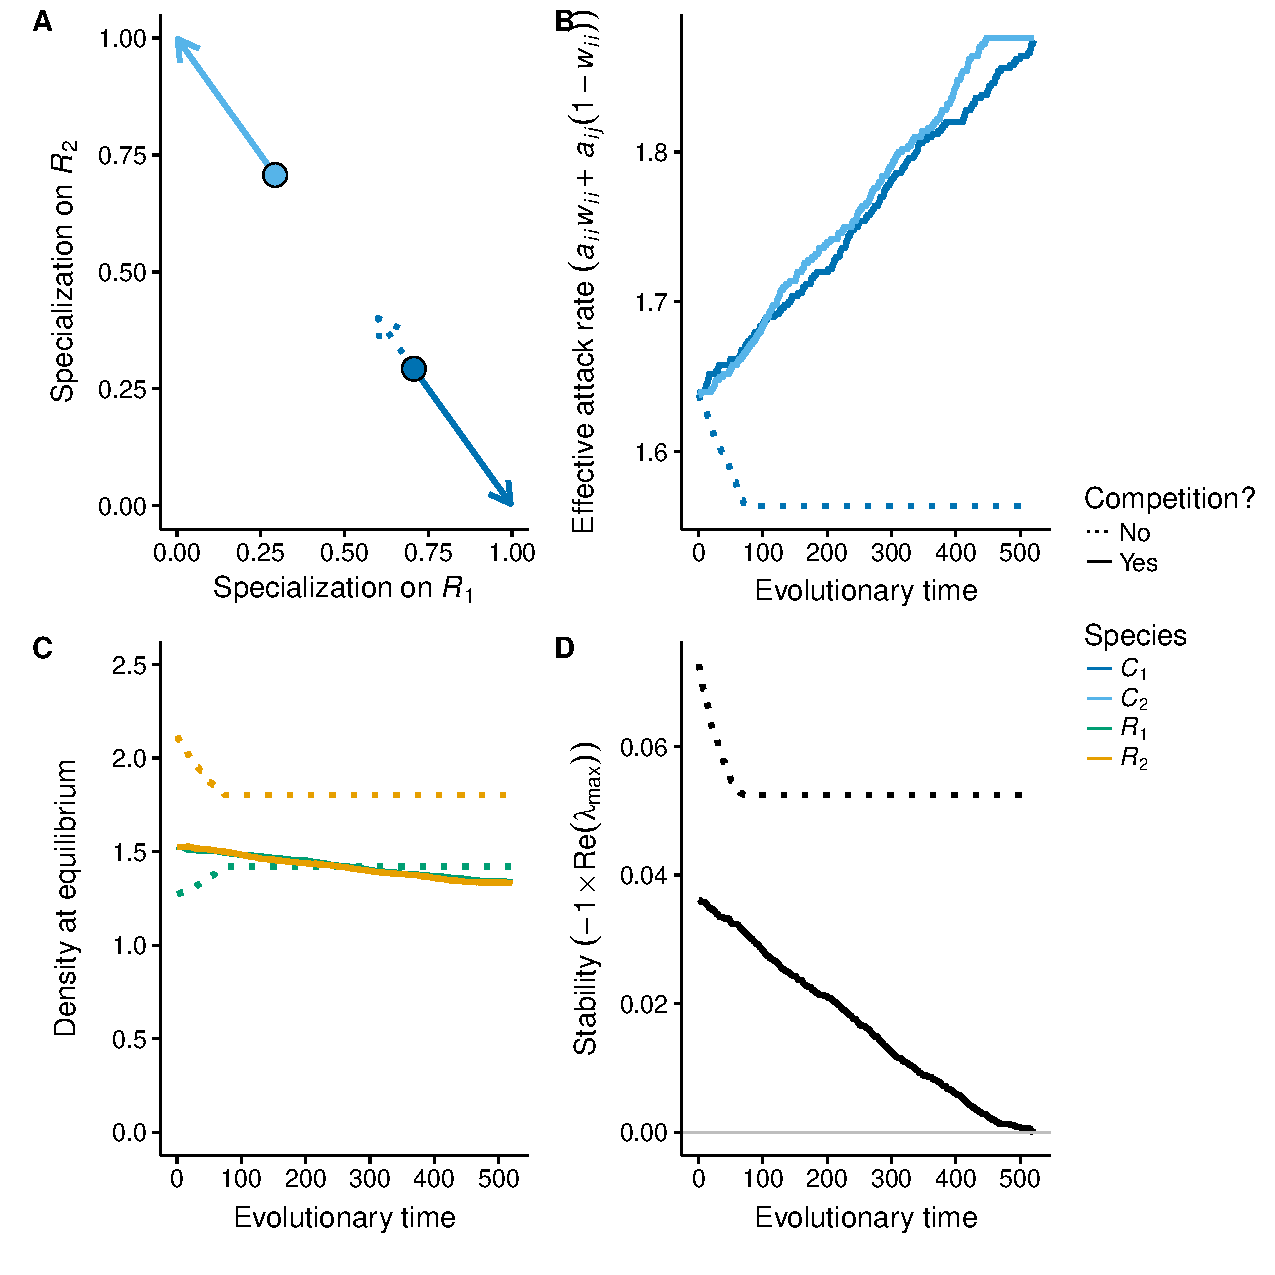
\includegraphics[scale = 0.6]{fig_theory.pdf}
\caption{Coevolution of competitors destabilizes a model food web. In the presence of a competitor, $C_2$, each consumer specializes on the resource it is pre-adapted to, whereas in the absence of competition, a consumer will evolve a generalist phenotype that can more equally exploit both resources (A). This ecological character displacement causes consumers to evolve a higher effective attack rate (B), which suppresses the density of both resources relative to the food web with no competing consumer (C). This enhanced resource exploitation with coevolving competitors results in a relatively less stable food web (D). The grey line in (D), where $-1\times \text{Re}(\lambda_{max})=0$, corresponds to the local stability boundary of the food web. Non-evolving model parameters for this simulation: $r=1$, $K=4$, $e=0.8$, $h=0.4$, $w=0.6$, $m=1$. Initial evolving parameters and species densities when "Evolutionary time = 0": $a_{ii}=1.93$, $a_{ij}=1.2$; $R_1=R_2=2$, $C_1=C_2=1$.}
\label{Fig:theory}
\end{figure}

\begin{figure}[ht]
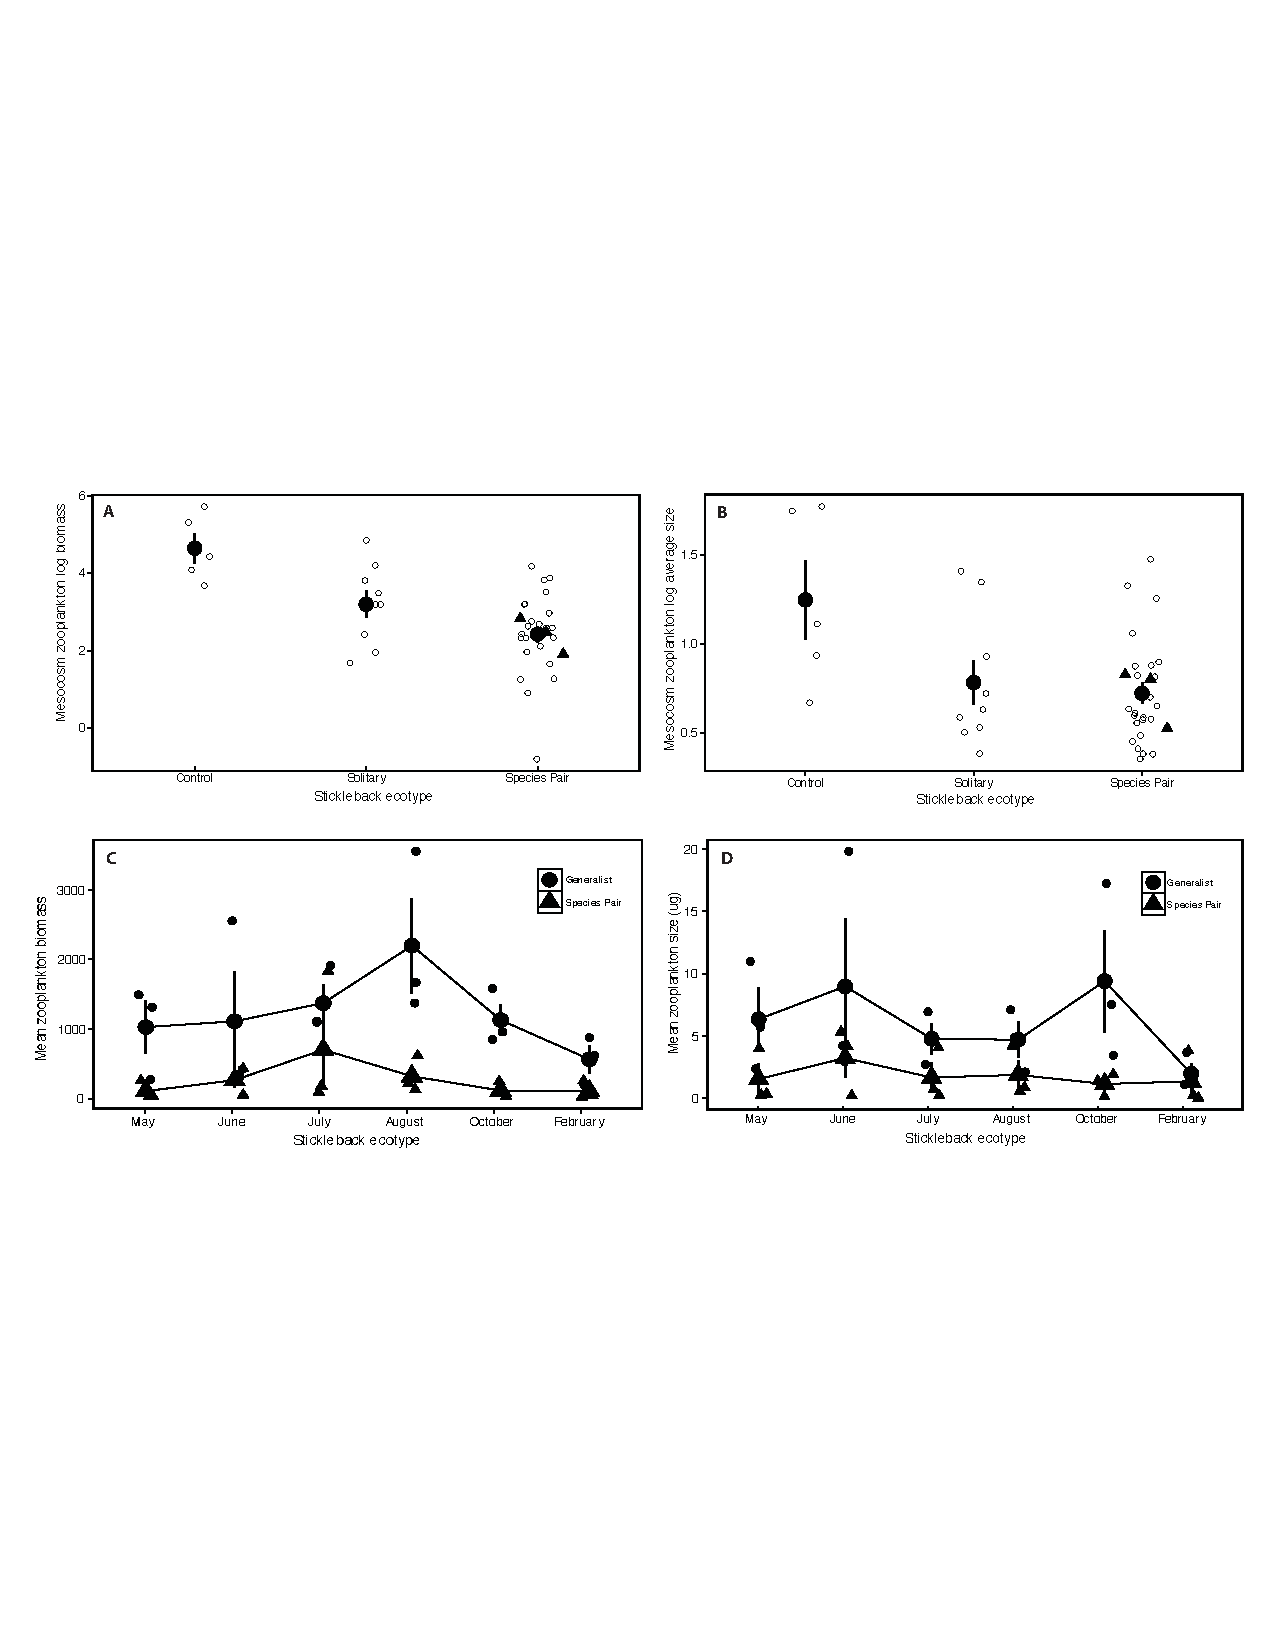
\includegraphics[trim=1cm 8cm 1cm 8cm, scale=0.8]{repeat_Fig1_161109.pdf}
\caption{Panels A and B illustrate the effects of stickleback speciation on log zooplankton biomass and average size from the mesocosm experiment.  Small triangles show the mean of each independently evolved species pair of stickleback.  Panels C and D show the effects of stickleback speciation on log zooplankton biomass and average size across the year from the field study.}
\label{Fig:Zoop}
\end{figure}

\newpage

\begin{figure}[ht]
%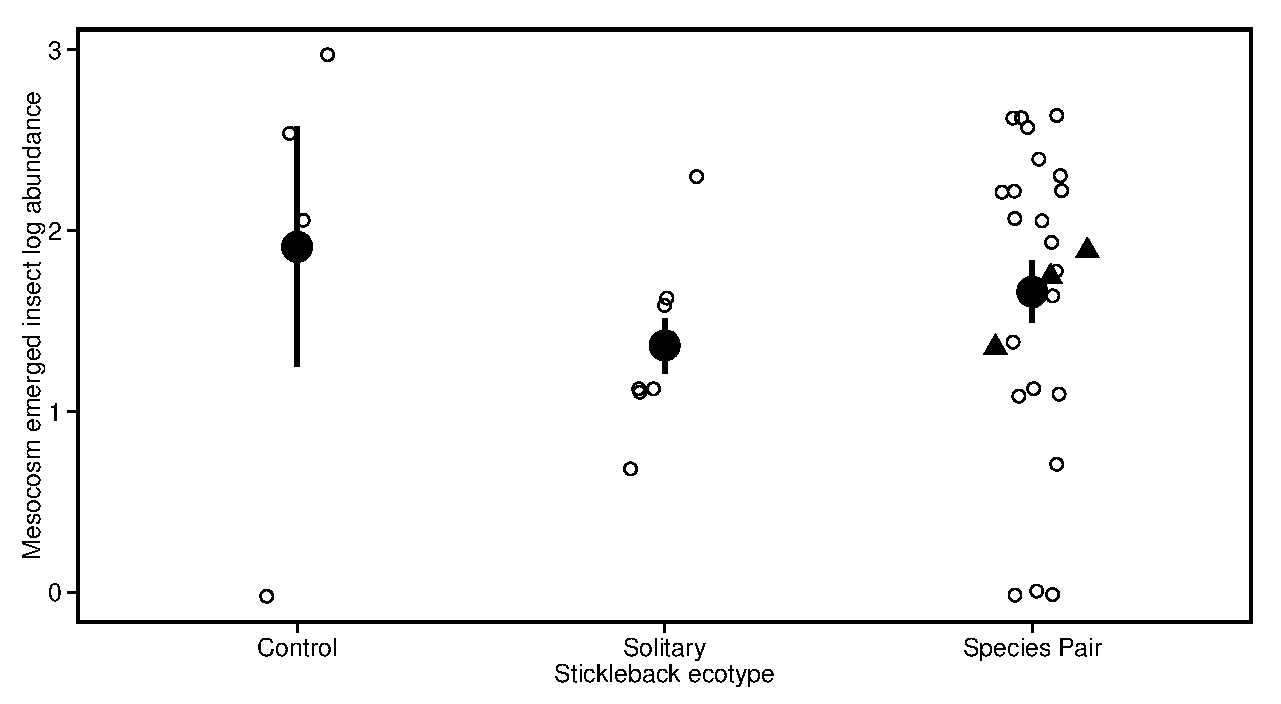
\includegraphics[scale = 0.3]{meso_EmergedLogAbun_160119.pdf}
%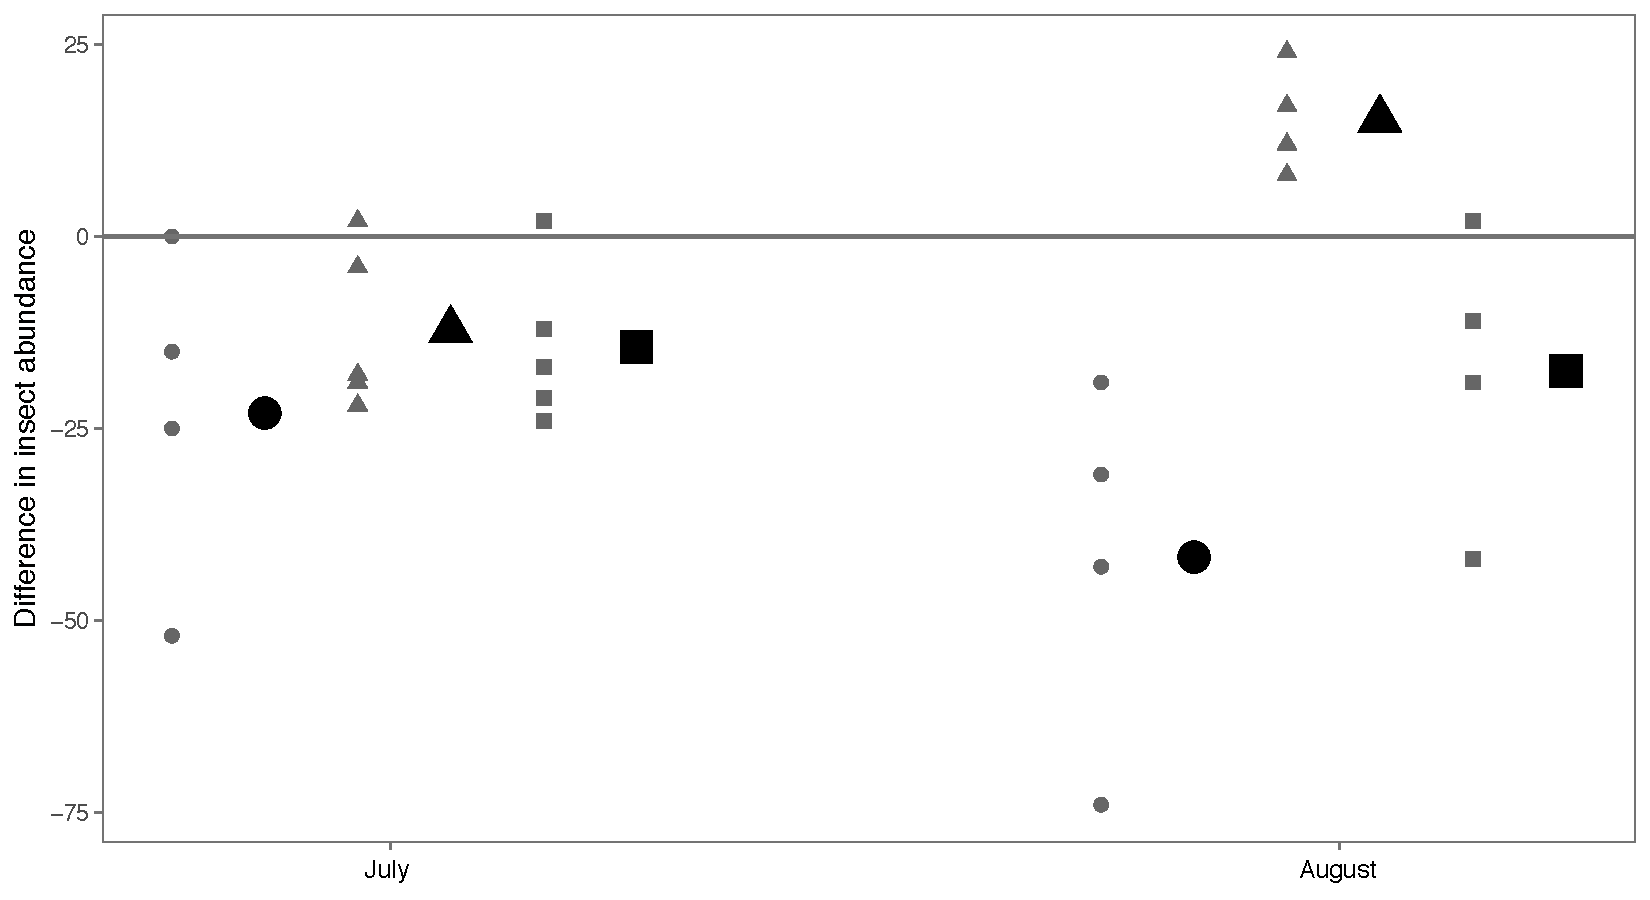
\includegraphics[scale = 0.3]{Field_Insect_Emerge_170403.pdf}
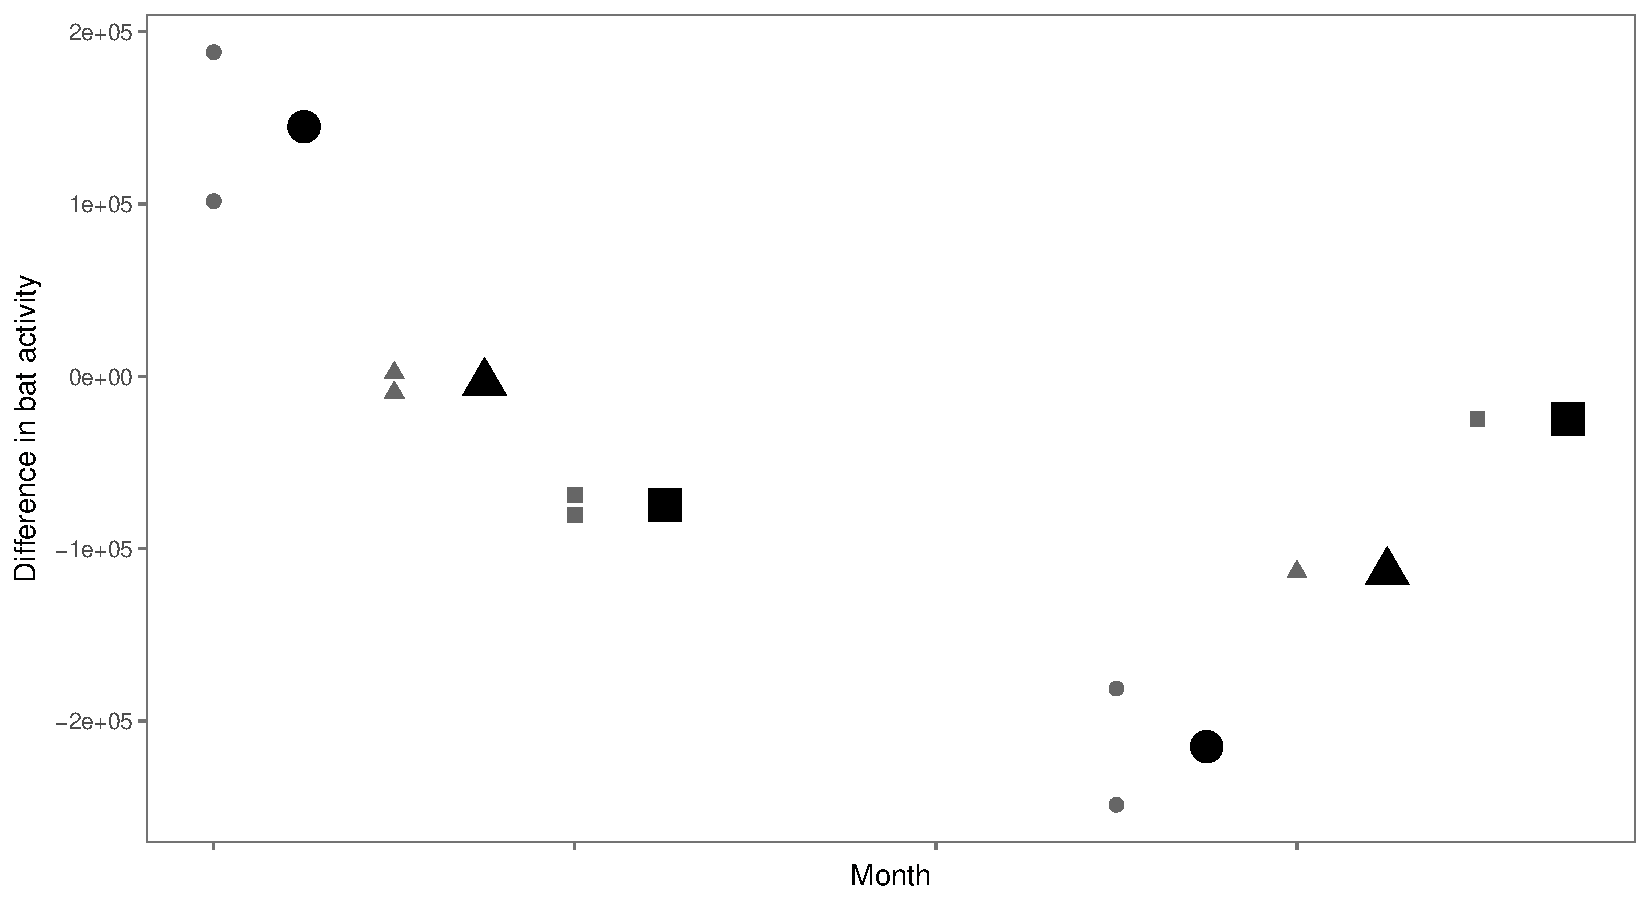
\includegraphics[scale = 0.4]{Field_Bat_170403.pdf}
\caption{Panel A shows the number of insects emerging from the aquatic environment in the mesocosm experiment.  Panel B shows the difference in insect emergence in observational field data between paired lakes, with negative values indicating greater emergence in the species pair lakes.  Panel C shows the difference in microchiropteran foraging activity between paired lakes, with negative values indicating greater foraging above species pair lakes.}
\label{Fig:AnotherFigure}
\end{figure}

%\subsection*{Online figure legends}

%\renewcommand{\thefigure}{A\arabic{figure}}
%\setcounter{figure}{0}

%\begin{figure}[h!]
%\includegraphics{jumps20m}
%\caption{\textit{A}, the quick red fox proceeding to jump 20~m straight 
%into the air over not one, but several lazy dogs. \textit{B}, the quick 
%red fox landing gracefully despite the skepticism of naysayers.}
%\label{Fig:Jumps}
%\end{figure}

%\begin{figure}[h!]
%\includegraphics{jumps-nr-okapi}
%\caption{The quicker the red fox jumps, the likelier it is to land near 
%an okapi. For further details, see \citet{LemKapEx07}.}
%\label{Fig:JumpsOk}
%\end{figure}

%\renewcommand{\thefigure}{B\arabic{figure}}
%\setcounter{figure}{0}

\end{document}
